\subsection{表达结合性与交换性的图表}

设 A 为一个交换环，E 为一个 A-模；给定一个 \(E \times E\) 到 E 中的双线性映射，相当于给定一个 A-线性映射：

\[
m: \mathbf {E} \otimes_ {\mathbf {A}} \mathbf {E} \rightarrow \mathbf {E}
\]

(II，§ 3，第 5 号)。因此，E 上的一个 A-代数结构由给出 E 上的一个 A-模结构以及一个 E \(\otimes_{\mathbf{A}}\) E 到 E 中的 A-线性映射来定义。

设 \(E'\) 是另一个 A-代数， \(m': E' \otimes_{A} E' \to E'\) 是定义 \(E'\) 的乘法的 A-线性映射。映射 \(f: E \to E'\) 是一个 A-代数同态，当且仅当 \(f\) 是使图表交换的映射

\[
\begin{array}{c} \mathrm{E} \otimes_ {\mathrm{A}} \mathrm{E} \xrightarrow {f \otimes f} \mathrm{E} ^ {\prime} \otimes_ {\mathrm{A}} \mathrm{E} ^ {\prime} \\ m \Biggl \downarrow \\ \mathrm{E} \xrightarrow {f} \mathrm{E} ^ {\prime} \end{array}
\]

A-代数 E 为结合的，必要且充分的条件是（考虑到张量积的结合性，参见 II，§ 3，第 8 号）A-线性映射的图表

\[
\begin{array}{c} \mathrm{E} \otimes_ {\mathrm{A}} \mathrm{E} \otimes_ {\mathrm{A}} \mathrm{E} \xrightarrow {m \otimes 1 _ {\mathrm{E}}} \mathrm{E} \otimes_ {\mathrm{A}} \mathrm{E} \\ \downarrow^ {1 _ {\mathrm{E}} \otimes m} \\ \mathrm{E} \otimes_ {\mathrm{A}} \mathrm{E} \xrightarrow {m} \mathrm{E} \end{array}
\]

是交换的。类似地，A-代数 E 为交换的，必要且充分的条件是 A-线性映射的图表

\[
\begin{array}{c} \mathrm{E} \otimes_ {\mathrm{A}} \mathrm{E} \xrightarrow {\sigma} \mathrm{E} \otimes_ {\mathrm{A}} \mathrm{E} \\ \Biggl \downarrow m \Biggl \downarrow m \\ \mathrm{E} \end{array}
\]

是交换的，其中 \(\sigma\) 表示由 \(\sigma(x \otimes y) = y \otimes x\) （对 \(x \in \mathbf{E}\) ， \(y \in \mathbf{E}\) ）定义的典范 A-线性映射（II，§ 3，第 1 号，命题 1 的推论 2）。

对所有 \(c \in \mathbf{E}\) ，用 \(\eta_c\) 表示由 \(\mathbf{A}\) 到 \(\mathbf{E}\) 的、由条件 \(\eta_c(1) = c\) 定义的 A-线性映射。 \(c\) 为 \(\mathbf{E}\) 的单位元，必要且充分的条件是下列两个图表

\pandocbounded{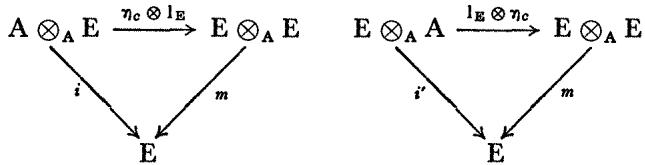
\includegraphics[keepaspectratio]{images/part003_ee0531f1.jpg}}

是交换的（其中 i 和 i' 表示典范同构（II，§3，第 4 号，命题 4））。

设 E 是一个具有单位元 e 的 A-代数，并设 \(\eta = \eta_{e}\) （也记作 \(\eta_{E}\) ）；则 \(\eta(\alpha\beta) = \eta(\alpha)\eta(\beta) = \alpha\eta(\beta)\) ，因为由（2）（第 1 号），

\[
(\alpha e) (\beta e) = (\alpha \beta) e = \alpha (\beta e);
\]

因此 \(\eta\) 是一个 A-代数同态。注意，E 上的 A-模结构可以利用 \(\eta\) 来定义，因为

\[
\alpha x = \eta (\alpha). x \quad \text { for } \alpha \in \mathrm{A}, x \in \mathrm{E}\tag{3}
\]

（其中右端的乘法在 E 中）。同态 \(\eta\) 的像是 E 的一个子代数，其元素与 E 的所有元素交换。同态 \(\eta\) 的核是 A-模 E 中元素 \(e\) 的零化子；由 (3)，它也是 A-模 E 的零化子（II，§ 1，第 12 号）。

当代数 E 含单位元且结合时， \(\eta\) 是一个环同态。反之，设 \(\rho:A\to B\) 是一个环同态，其像 \(\rho(A)\) 包含在 B 的中心内，并设环 A 交换；则在 B 上定义了一个结合且含单位元的 A-代数结构，其定义式为（参见 (3)）

\[
\lambda x = \rho (\lambda). x \quad \text { for } \lambda \in \mathbf {A}, x \in \mathbf {E}.
\]

